\chapter{相关理论及技术}
本章首先对文本分类任务进行简单介绍以及单词嵌入表示如word2vec,glove等学习方式。本章主要围绕了基于图模型文本分类模型的相关理论以及关键技术。包括图模型,图卷积神经网络(GCN),注意力机制,以及本文将会使用的技术和深度学习模型如TF-IDF、GRU、CNN、Bert等。
\section{文本分类任务}
在如今人类活动中产生了大量的文本数据,如美团、大众点评上对美食的各类评论,豆瓣上对书籍、电影的评价,以及人类历史活动中各类简短信息,例如微博、推特,新闻摘要等。这类都是一些短文本,对这类短文本进行分析一方面有助于实现快速归类,对于不同类型的文本内容进行整理;
另一方面针对用户的平均分析用户行为,改善服务。文本分类涉及多种情况,本文主要探讨整体文本分类算法以及方面级情感分析算法。
\subsection{整体文本分类和方面级情感分析}
(1)整体文本分类

对于整体文本分类来说,目的是对整段文本的描述进行判断,以数据集R8为例,该数据集为分类任务常用的文本数据集,为路透社新闻文本,共有八个分类。

\begin{figure}[htb]%\small tbp
	\setlength{\belowcaptionskip}{0pt}
	\centering
	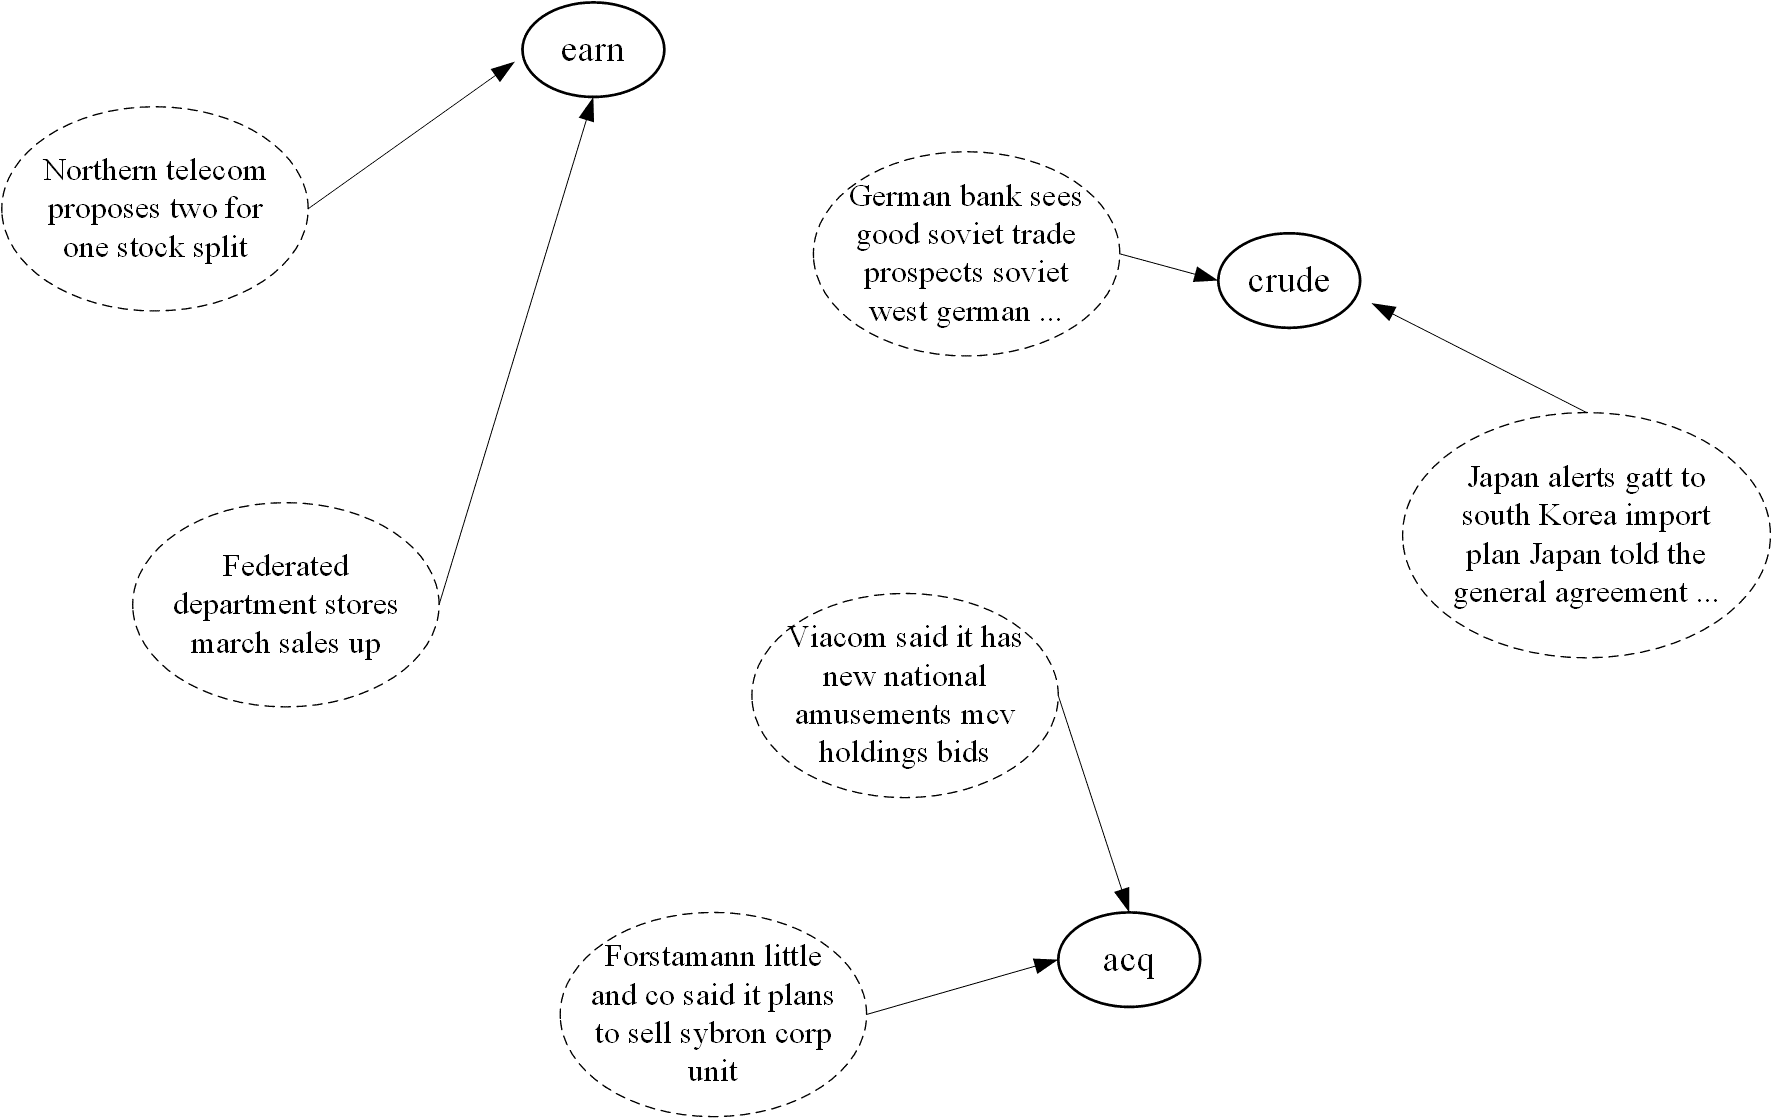
\includegraphics[width=0.8\textwidth]{pic/2-1.png}
	\caption{R8数据集}
	\label{R8datasets}
\end{figure}
如图\ref{R8datasets}所示,截取了数据集中三个分类标签,分别是earn、acq和crude。每个类别下都有对应的文本,代表了这个文本的分类属于这个标签。
从图\ref{R8datasets}可以看出来,整体文本分类任务是对整句话进行分类,一般一个文本只属于一个类别。比如“Federated department stores march sales up”这句话,
从文意可以看出描述了联邦百货公司3月销售额上升,正好符合earn标签的含义,因此对于这段文本可以分类为earn。
总的来说,本文定义的整体文本分类任务是针对于一个文本整体进行分类,判断该段文本从属的标签类别,一般情况下一个文本只有一个标签。

(2)方面级情感分析任务

方面级情感分析任务不同于整体文本分类任务,它是对文本中存在的方面目标词进行分类,而不是整段文本,因此,一段文本,对于方面级情感分析任务来说,存在多个方面目标词,那么就可能存在多个类别标签。方面目标词即可以是一个单词也可以是一个词组。本文以semeval14数据集为例,该数据集是14年推特的文本数据集,常用来做情感分析。
\begin{figure}[htb]%\small tbp
	\setlength{\belowcaptionskip}{0pt}
	\centering
	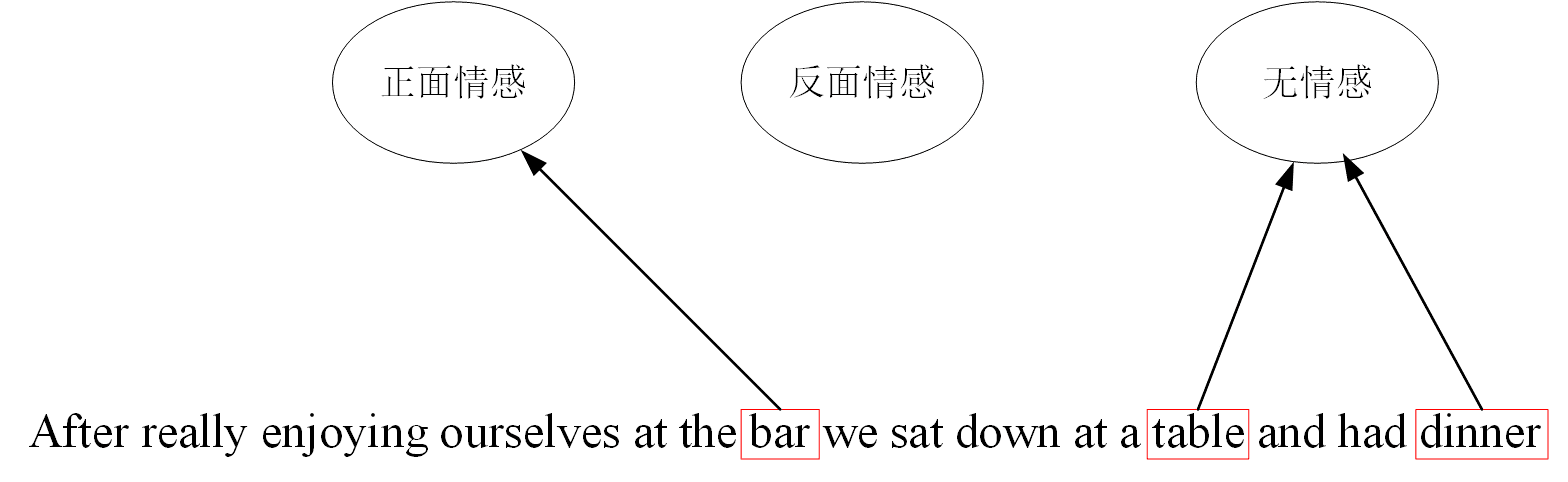
\includegraphics[width=0.8\textwidth]{pic/2-2.png}
	\caption{semeval14数据集}
	\label{semeval14datasets}
\end{figure}

从图\ref{semeval14datasets}可以看出,该段文本共有三个由红色方框标注出来的方面目标词,分别是‘bar’、‘table’、‘dinner’。
方面级情感分析任务就是需要实现分别对这三个词的情感进行分析,而不是对整个文本进行分类。因此相比于整体文本分类任务来说,需要更精细的设计。比如‘bar’这个词,从文本描述来看,最能体现这个词语情感信息的词应该是‘enjoying’,而‘enjoying’代表了正面的情感,因此对于‘bar’这个方面目标词把它归于‘正面情感’这个标签;对于‘table’和‘dinner’,这句话没有明显的情感,仅仅作为描述语句或是补充,因此没有特别的情感色彩,把它们归属于‘无情感’的标签下。所以,对于方面级情感分析任务来说,需要根据方面目标词进行分析,把握该词汇与其他具有情感色彩的词汇之间的关系,分析具体的情感色彩指代。
同一个句子中可能存在多个情感色彩词,并且词的含义可能是相反的,一个可能代表了积极正面的情感,另一个可能是消极的负面情感。相比于整体文本分类任务来说,更具有难度。
\section{单词嵌入表示}
文本数据不同于一般的图像、音频等数据。图像数据本身就具有意义,是天然带有的属性,即使没有经过训练的生物或许也能分辨不同的图片。而文本数据是人类的高层的抽象的思维信息表达的工具,具有高度抽象特征。在图像处理中,一张图片通常可以用一个矩阵表示,其中每个坐标的点即为像素点的值,矩阵中每个数值都具有一定意义,且矩阵属于稠密矩阵。而一段文本通常有多个单词构成,每个单词可以由一个向量表示,如图\ref{textEmb}所示。
\begin{figure}[htb]%\small tbp
	\setlength{\belowcaptionskip}{0pt}
	\centering
	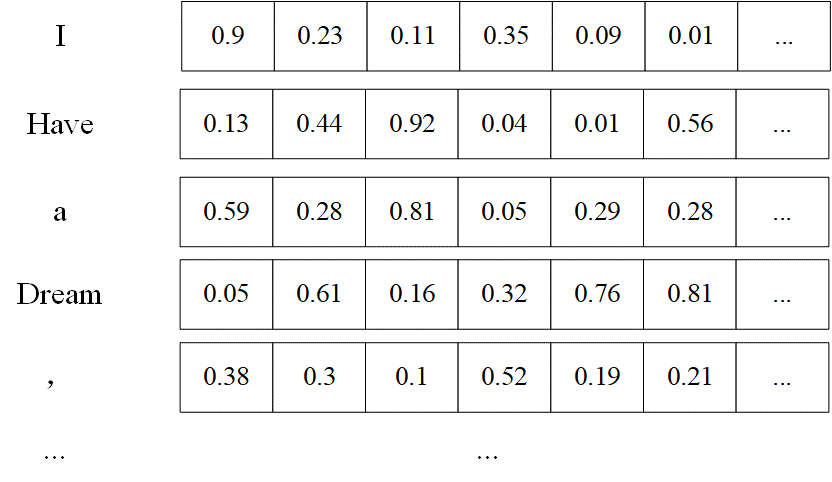
\includegraphics[width=0.8\textwidth]{pic/2-3.png}
	\caption{文本向量表示}
	\label{textEmb}
\end{figure}

如图\ref{textEmb}所示,一句话由多个向量组成,每个单词有一个向量表示,不同于图片矩阵,向量中的每个单一的值没有具体的含义,所有的值构成一个向量才具有表示为单词信息的含义。向量中的值一般取决于表示的方法。如采用one-hot的表示方式,向量中仅含有一个为1的值,其他值为0。向量的维度由单词个数决定,如一个单词量为2000的词库,构成的单词向量即为1*2000的向量。如单词Dream位于该词库中第二个位置,它的向量表示可能是(0,1,0,0,…,0),另一个单词Have可能位于第1000个位置,那么它的向量表示可能就是(0,0,…,1,…,0,0)。每个单词都由一个唯一的向量表示。虽然这种方式非常简单,但同时带来许多问题。1.向量维度随着单词数量而增加,当面对几万甚至几十万的词库时显得力不从心。2.每个单词向量都仅仅由0,1构成,没有具体含义,难以把握单词之间的联系。

Hinton提出的Distributed Representation\citing{hinton1986learning}思想可以用以学习词向量解决这个问题。这类词向量的表示一般类似于(0.22,-0.17,…,0.65,0.01)这种。而现如今常用的学习词向量的方法有word2vec,glove等。

Word2vec它采用了一个两层神经网络的基础架构,采用CBOW或是Skip-gram的模型训练文本单词,挖掘单词语义,将单词嵌入到一个高维的向量表示空间,最终获得每一个单词的一个向量表示。
\begin{figure}[htb]%\small tbp
	\setlength{\belowcaptionskip}{0pt}
	\centering
	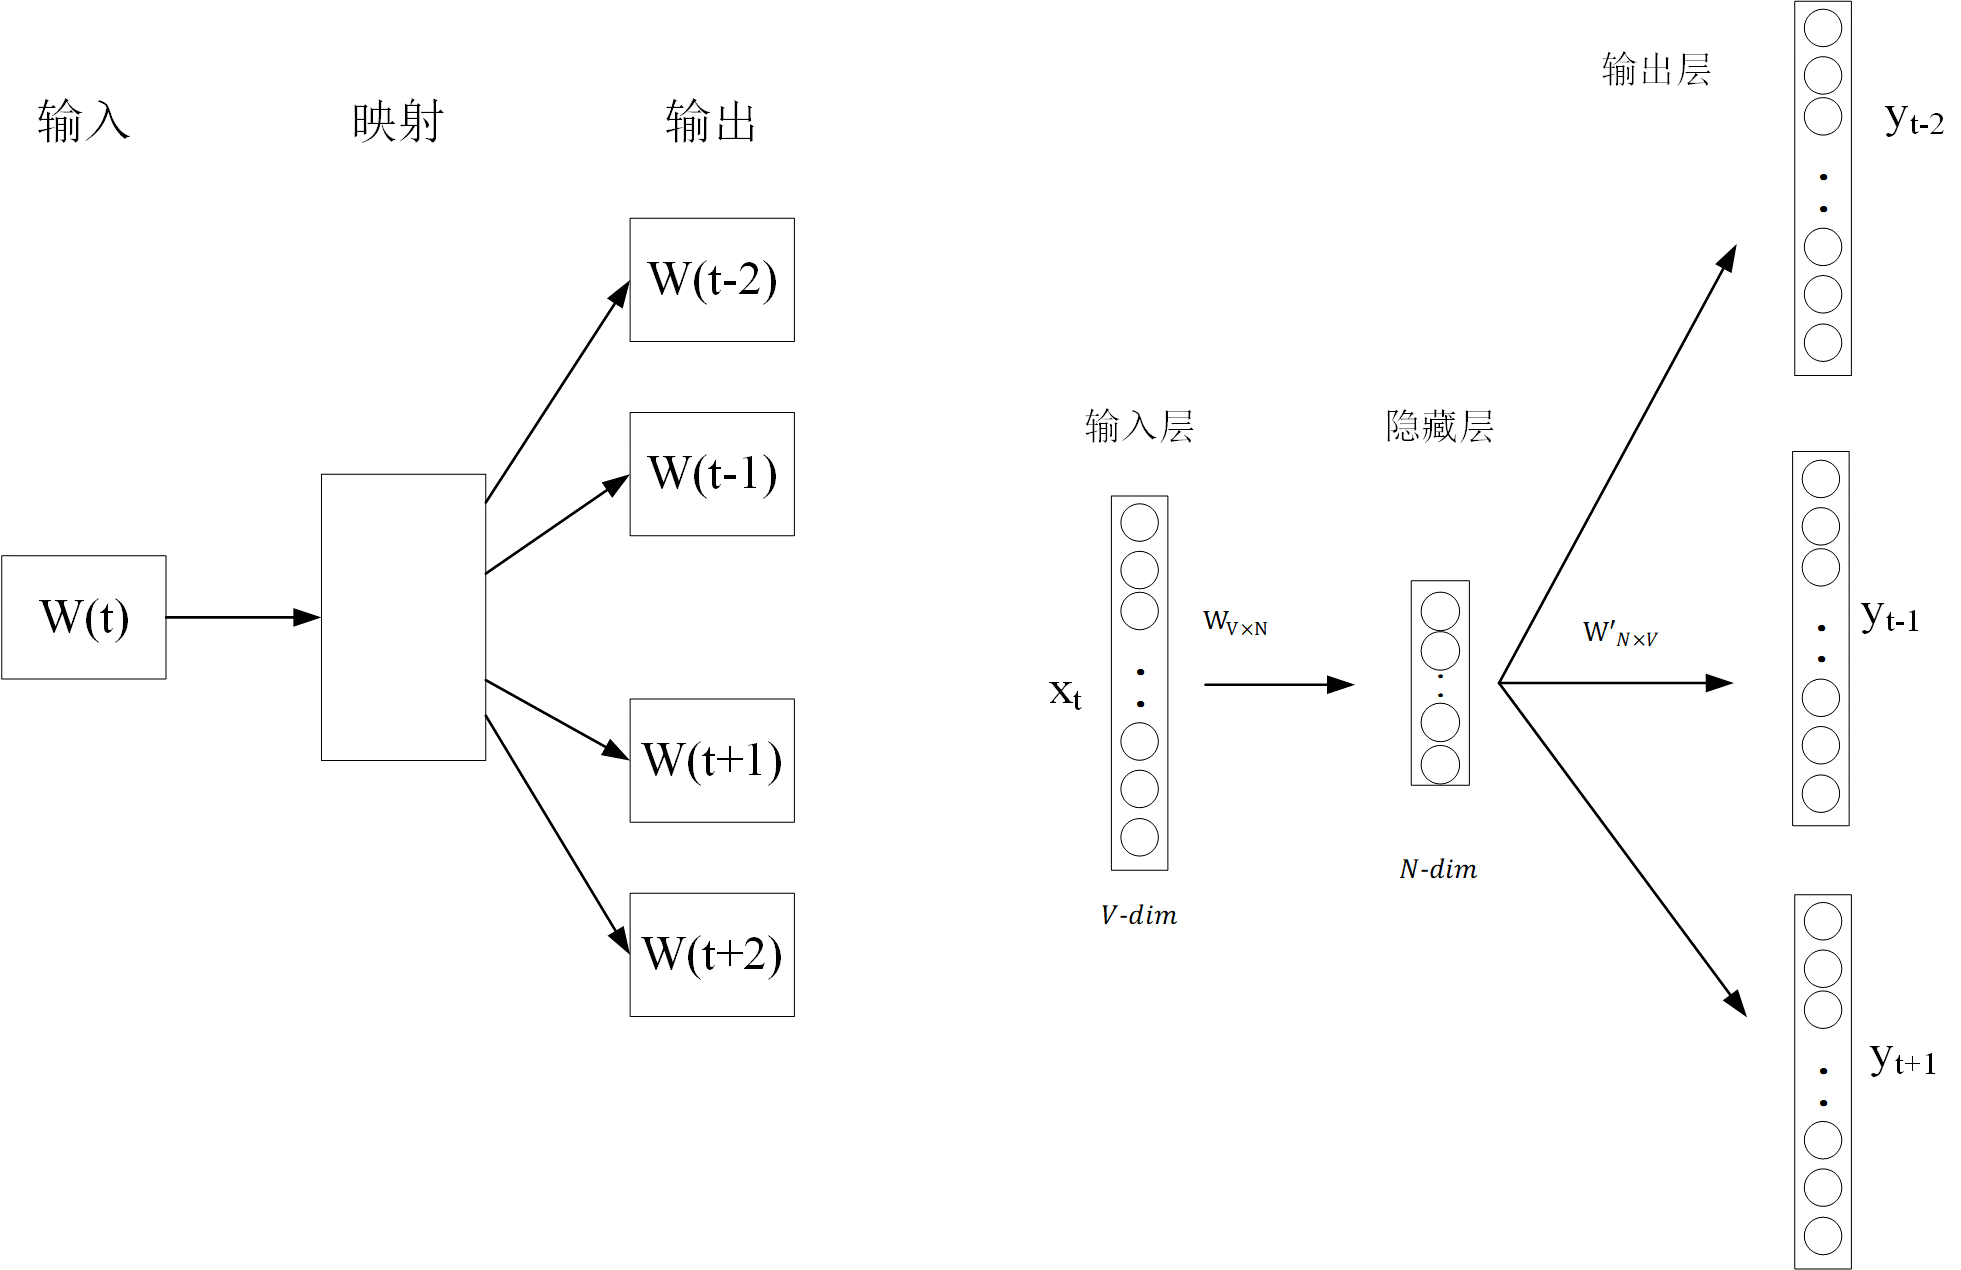
\includegraphics[width=0.8\textwidth]{pic/2-4.png}
	\caption{skip-gram模型}
	\label{skip-gram}
\end{figure}

Skip-gram模型如图\ref{skip-gram}所示,图左为模型架构,即通过中间单词预测该单词的上下文词。神经网络模型如图右所示。Skip-gram训练模型仅包含一个没有激活函数的隐藏层,和使用softmax激活函数的输出层。对于一个包含V个单词的数据集,模型的输入是一个V维的one-hot向量,经过一个$W_{V\times N}$的矩阵转化为N维的向量$h_t$,通常N远远小于V,这样一来可以将单词维度下降到很小,而所谓的$W_{V\times N}$参数矩阵即是我们需要学习的词嵌入矩阵。之后在经过一个${W^\prime}_{N\times V}$的参数矩阵,将隐藏向量$h_t$转为一个V维的向量,经过softmax激活函数,向量中的每个值都在0-1之间,代表着预测的单词的概率。计算公式如下:
\begin{equation}\label{skip-gramFormula1}
	h_t=Wx_t
\end{equation}
\begin{equation}\label{skip-gramFormula2}
	u_{t-1}=W^{\prime}h_t
\end{equation}
\begin{equation}\label{skip-gramFormula3}
	p\left(w_{t-1}\middle|w_t\right)=y_{t-1}=\frac{exp\left(u_{t-1}\right)}{\sum_{j=1}^{V}exp\left(u_j\right)}
\end{equation}
其中$W$,$W^\prime$分别为$V\times N$维,$N\times V$维的参数矩阵,$p\left(w_{t-1}\middle|\ w_t\right)$表示单词$w_t$的上下文预测单词$w_{t-1}$的概率。
\begin{figure}[htb]%\small tbp
	\setlength{\belowcaptionskip}{0pt}
	\centering
	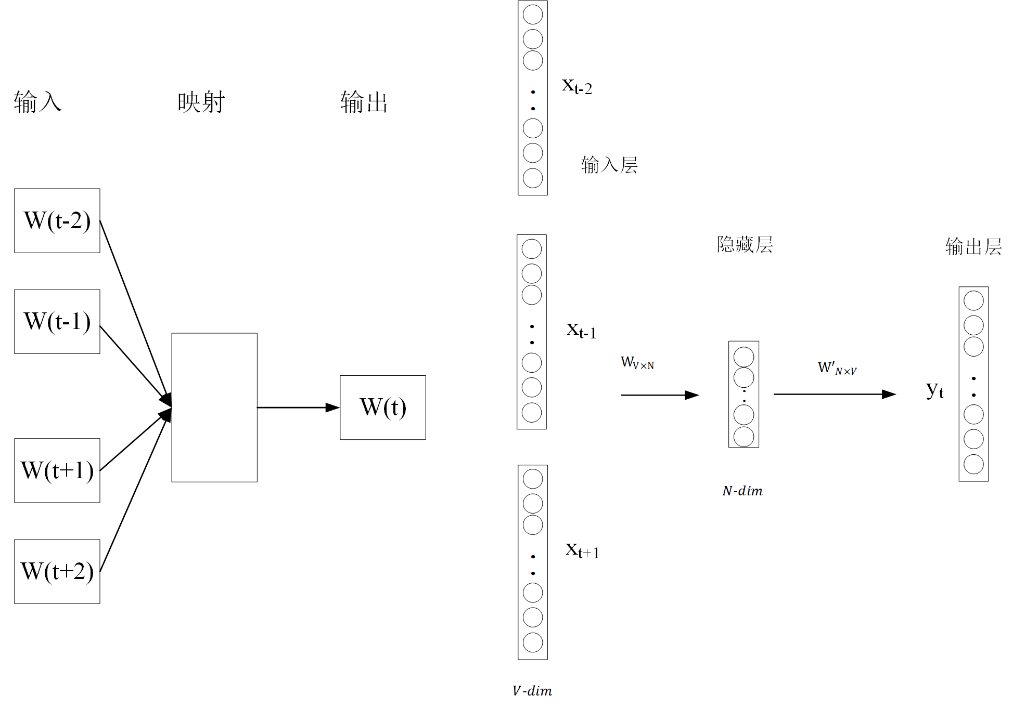
\includegraphics[width=0.8\textwidth]{pic/2-5.png}
	\caption{CBOW模型}
	\label{CBOW}
\end{figure}

CBOW模型如图\ref{CBOW}所示,图左为COBW模型架构,它与skip-gram相反,通过上下文信息预测中间词。首先是通过上下文多个单词计算隐层向量$h_t$,计算公式如\ref{CBOWFormula1},主要采用上下文C个单词的加权和得出。接着与skip-gram类似通过输出层转化为V维向量,再通过softmax预测。
\begin{equation}\label{CBOWFormula1}
	h_t=\frac{1}{C}W\sum_{i=1}^{c}x_i
\end{equation}

Glove方法也是一种学习单词表示的方法。他与word2vec类似,采用一个大型的语料库进行训练,将单词嵌入到高维空间,实现用一组向量表示单词。但是word2vec的CBOW和skip-gram方法是基于局部上下文窗口的,忽略了单词之间的共现信息。Glove方法的提出,考虑了这种全局词汇的共现信息,并且结合局部上下文窗口的方法的优点,来学习词向量,相比word2vec效果得到了一定的提升。
Glove目标函数可以近似为:
\begin{equation}\label{CBOWFormula1}
	F\left(w_i-w_j,w_k\right)=\frac{p_{ik}}{p_{jk}}
\end{equation}
其中$w_i$,$w_j$,$w_k$分别代表单词i,j,k的表示向量,$p_{ik}$代表单词k出现在单词i上下文的概率。Glove的目标就是找到函数F的表示空间,从而得到所有单词的向量表示。
\section{图模型相关理论}
现实生活中存在着大量的图结构数据,比如分子结构,社交网络,地理位置。这些数据的关键点在于都有一个可抽象化的节点,比如社交网络中的用户,以及连接这些节点的边即关系,比如社交网络中用户的关注、用户的点赞评论等交互。如何去利用这些图数据那就首先需要获取这些图数据中节点或是边的有效表示\citing{hamilton2017representation}。现如今已有大量关于图模型数据处理的研究\citing{scarselli2008graph,battaglia2016interaction,zhang2018end}。

图神经网络(GNN)主要是利用神经网络去学习节点表示$h_v$,或是整个图的向量表示$h_G$。通常每个节点v会有一个初始的向量表示$x_v$,经过图模型计算学习获得新的表示。而学习的过程主要是一种信息聚集的过程,即节点首先会从自己的邻居节点聚集信息,随着每一轮的聚集,当前节点将会获取到更远处节点的信息,即经过k轮迭代,当前节点或许可以得到k-跳的邻居节点信息,如下公式所示:
\begin{equation}\label{GNNFormula1}
	a_v^kf=\left(h_u^{k-1}:u\in\mathcal{N}\left(v\right)\right)
\end{equation}
\begin{equation}\label{GNNFormula2}
	h_v^k=g\left(\left[h_v^{k-1},a_v^k\right]\right)
\end{equation}

其中k表示第k次聚集,$a_v^k$表示节点v从其邻居节点集合$\mathcal{N}\left(v\right)$聚集得到的信息。聚集过程可以采用简单的加权和,也可以根据算法自定义方式。主要功能就是将邻居节点的信息融合得到一个新的向量,即得到一个具有丰富信息的向量。随后节点v再将上一次迭代获取的到的向量表示与当前聚集轮次获得到的邻居信息融合起来,组成新的该节点的向量表示。随着次数的增多,当前节点将会获取到多跳邻居节点的信息,使得当前节点的向量表示更加丰富,融入了多种信息,表达更加全面。

\subsection{图卷积神经网络}
Kipf提出的图卷积神经网络\ref{kipf2016semi}是一种直接在图上进行计算的半监督学习模型。首先定义一个图$G=(V,E)$,其中$V\left(\left|V\right|=n\right)$表示图中的节点,共有n个,E表示图中的边的集合。如图\ref{topoFig}所示每个节点都与其他某个或多个节点进行相连,构成了一个拓扑图。可以用邻接矩阵$A$表示节点之间的关系,如图\ref{adjA}所示。其中两个节点之间如果有边,则矩阵对应位置的值为1,反之则为0。此外邻接矩阵对应的度矩阵$D$如图\ref{digD}所示。其中$D_{ij}=\sum_{j}\ A_{ij}$。
\begin{figure}[htb]%\small tbp
	\setlength{\belowcaptionskip}{0pt}
	\centering
	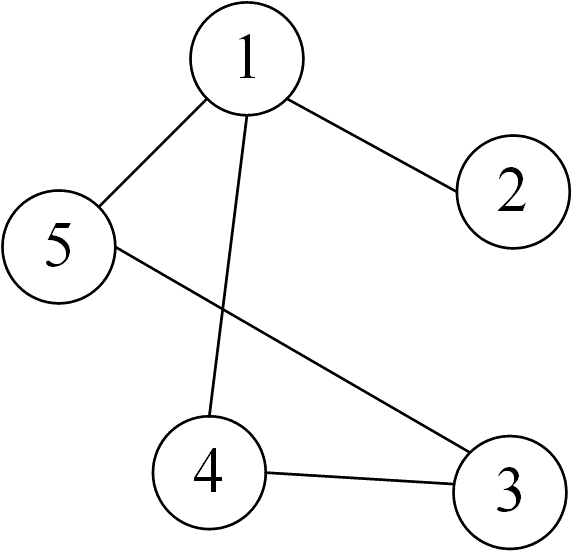
\includegraphics[width=0.4\textwidth]{pic/2-6.png}
	\caption{拓扑图}
	\label{topoFig}
\end{figure}
\begin{figure}[htb]%\small tbp
	\setlength{\belowcaptionskip}{0pt}
	\centering
	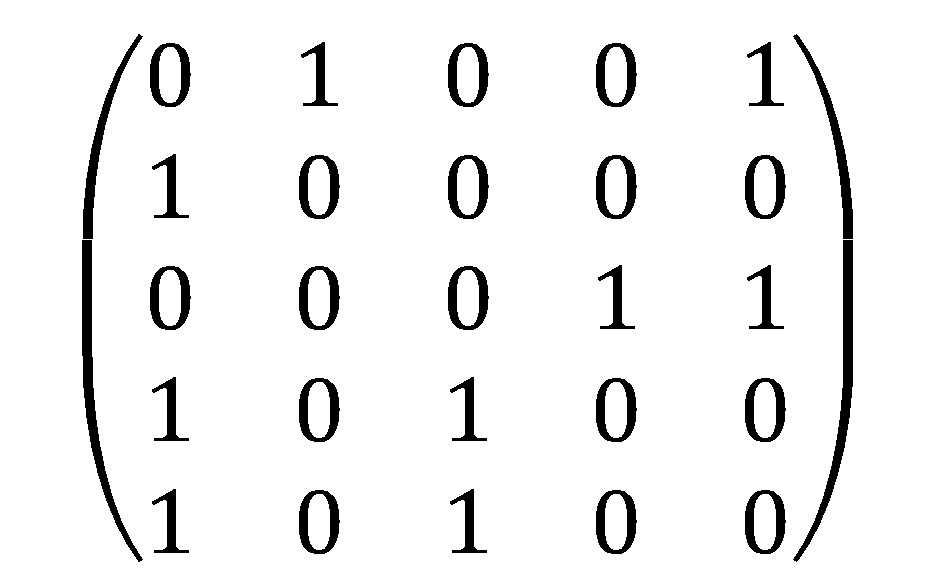
\includegraphics[width=0.4\textwidth]{pic/2-7.jpg}
	\caption{邻接矩阵A}
	\label{adjA}
\end{figure}
\begin{figure}[htb]%\small tbp
	\setlength{\belowcaptionskip}{0pt}
	\centering
	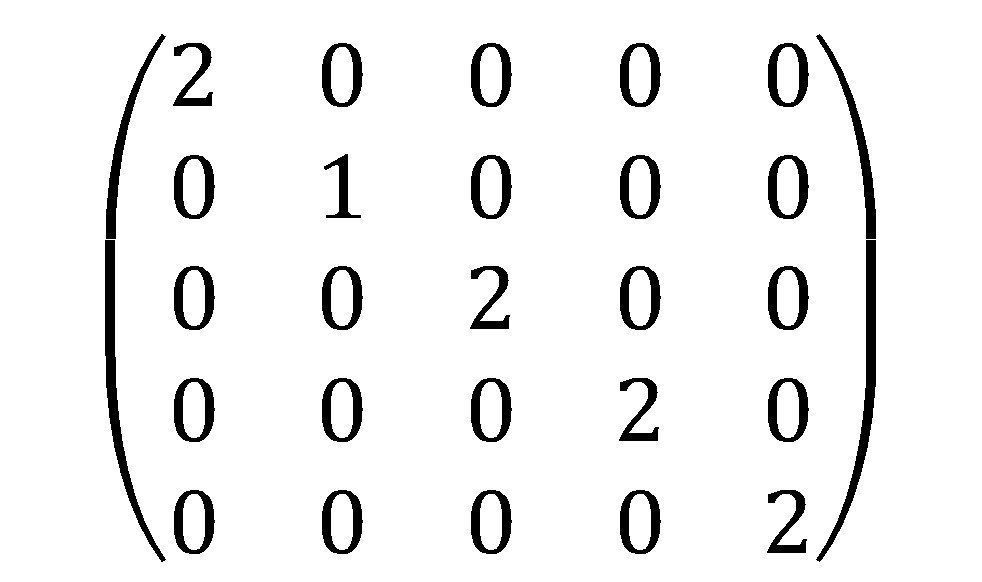
\includegraphics[width=0.4\textwidth]{pic/2-8.jpg}
	\caption{度矩阵D}
	\label{digD}
\end{figure}

假设每个节点$v_i$具有$m$维的特征向量$x_i\in R^m$,因此n节点构成特征向量矩阵$X\in R^{n\times m}$。节点信息在图中的传播主要沿着边进行,即通过边将每个节点的潜在信息进行传递。一个节点获取到来自其他节点的信息,将这些信息进行融合更新自身节点的信息,从而使得当前节点的信息更加丰富。每一次的信息传递都会增加额外的节点信息。刚开始,只会获取得到与当前节点直接相连的其他邻居节点的信息,同理邻居节点也会获取得到其邻居节点的信息,随着传递次数的增加,当前节点获取到的信息不仅仅是直接相邻的节点信息,更能获取得到更远的不相邻节点的信息。Kipf提出的图卷积计算方式可以由下公式得到:
\begin{equation}\label{GNNFormula1}
	H^{\left(l+1\right)}=\sigma{{(\hat{D}}^{-\frac{1}{2}}\hat{A}\hat{D}}^{-\frac{1}{2}}H^{\left(l\right)}W^{\left(l\right)})
\end{equation}

其中$\hat{A}=A+I$, $I$表示为单位矩阵。在原始的邻接矩阵上加上单位矩阵就是为了确保节点每次传递都能考虑到自身的信息。$H^{\left(l\right)}$表示为第$l$层的节点向量表示,$W^{\left(l\right)}$表示为第$l$层的参数。$\hat{D}$为$\hat{A}$的度矩阵。

\section{注意力机制}
\begin{figure}[htb]%\small tbp
	\setlength{\belowcaptionskip}{0pt}
	\centering
	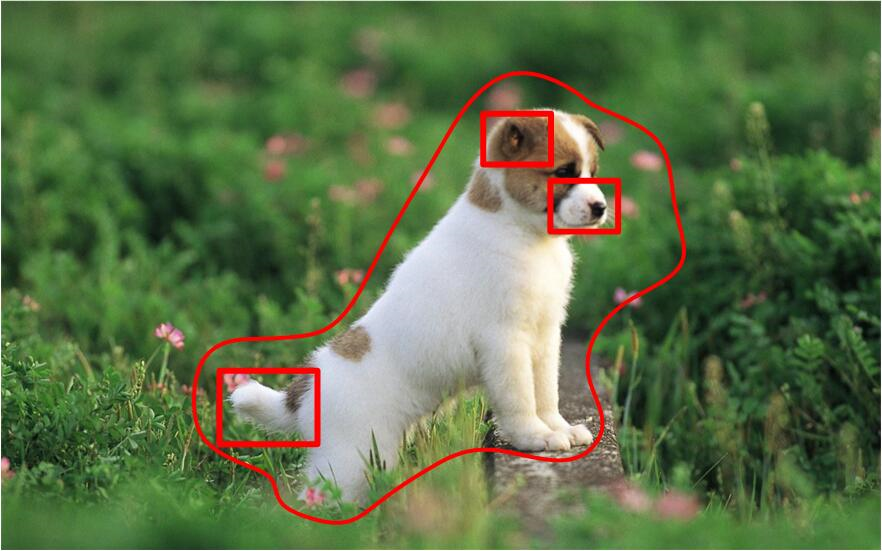
\includegraphics[width=0.6\textwidth]{pic/2-9.png}
	\caption{人类观察狗狗图}
	\label{watchDog}
\end{figure}
注意力机制就是模拟人类对视觉的处理,是源于对人类视觉的研究。人类通过眼睛观察周围场景,能够从有限的时间中快速挖掘场景中的信息,正是由于人类大脑提供的处理机制-注意力机制,让人能在复杂的场景中快速适应。人类对场景观察时,大部分情况下仅关注于重点区域,将大部分注意力资源都投入到这些区域中,而尽量忽略一些无关紧要的信息,实现资源的有限分配。这是人类与生俱来的赖以生存的机制,人类视觉的注意力机制大大提高了视觉信息处理的时效性以及准确性。如图\ref{watchDog}所示,人类对于图片的识别时,识别这张图像是猫还是狗,首先可能会把观察重点放在图片中存在的那个动物上,然后忽略图片中其他的场景,如图中红色线框所示,人类观察时,忽略了这个动物存在的场景,即忽略了周边的花草,因为这些信息对分析这个动物类别没有帮助。
确定了大致区域后,视觉进一步将注意力放在耳朵,嘴巴,尾巴等位置上,从这些有限的区域就能大致分析出这个动物属于狗,而不是猫。因此,注意力机制对于实现有限的资源调度以及提升准确率(因为避免了类似花草场景的干扰)具有很大帮助。

注意力机制之前主要大量用于视觉处理,首次用于自然语言处理领域可以追溯到Bahdanau\citing{bahdanau2014neural}等人在2014年提出的基于RNN的编码-解码翻译模型。该篇文章不同于以往的翻译模型—在编码阶段将所有单词编码为单一向量$c$,这样的处理方式会使得模型在压缩的信息的过程中不得不忽略一些信息,从而使得翻译模型在面对长句子时处理能力很差。Bahdanau并没有固定编码向量$c$,而是根据解码层每一步的隐藏状态与编码时每个单词的隐藏向量计算得到不断变化的编码向量$c_i$。这种技巧就是一种注意力机制的处理方式,大大提高了模型的性能。
\begin{figure}[htb]%\small tbp
	\setlength{\belowcaptionskip}{0pt}
	\centering
	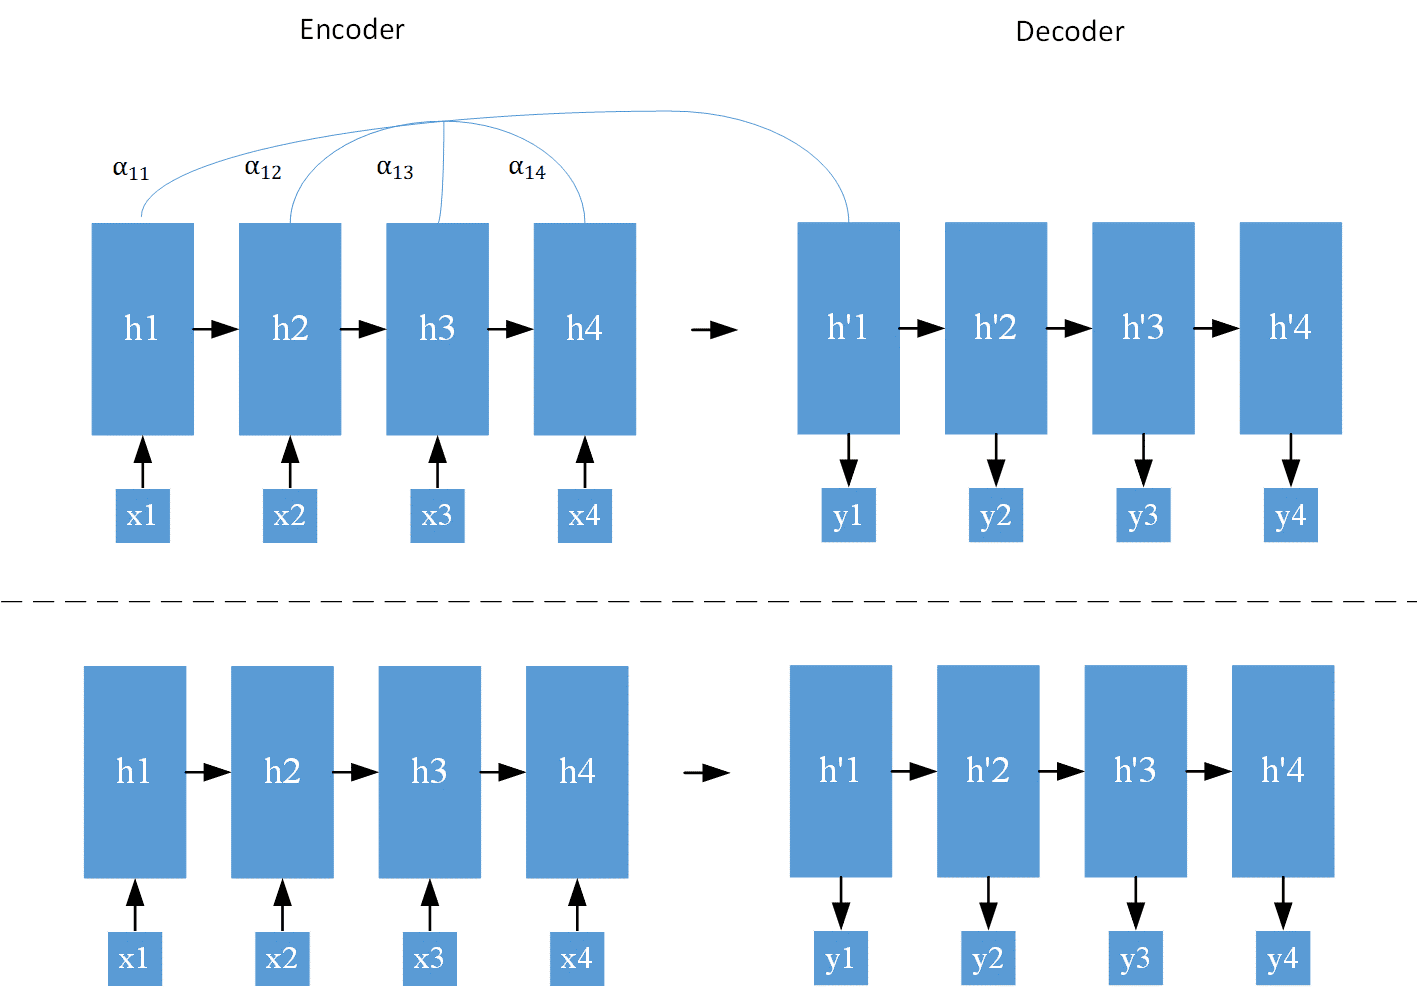
\includegraphics[width=0.8\textwidth]{pic/2-10.png}
	\caption{注意力机制RNN(上)与普通RNN(下)}
	\label{rnn-att}
\end{figure}

如图\ref{rnn-att}所示就是采用了注意力机制(图上)和普通RNN模型(图下)的差异。以下介绍几种常用的注意力机制使用方式。
\subsection{注意力机制计算}
在深度学习模型中,注意力机制计算可以简化为三类向量,一个是查询向量,即query向量,简称为$q$;一个是关键词向量,即key向量,简称为$k$;最后一类是值向量,即value向量,简称为$v$。通常查询向量$q$是一种特定于任务的向量,例如在上文提到的翻译模型中,$q$就是上一个隐藏状态向量。而$k$向量便是用来计算注意力分数的向量,如上文提到的翻译模型中的单词隐藏向量。$v$向量便是最终用于加权求和的向量。

注意力机制实现过程主要由以下公式计算得到\ref{attFormula1}、\ref{attFormula2}、\ref{attFormula3}。
\begin{equation}\label{attFormula1}
	a_i = score(q,k_i)
\end{equation}
\begin{equation}\label{attFormula2}
	\alpha_i = \frac{exp(a_i)}{\sum_{j}exp(a_j)}
\end{equation}
\begin{equation}\label{attFormula3}
	c=\sum_{j}v_j* \alpha_j
\end{equation}

其中$score(q,k_i)$为根据关键向量$k_i$与查询向量$q$计算得到的注意力分数,有不同的计算方式。
luong\citing{luong2015effective}提出公式\ref{scoreFormula1}和\ref{scoreFormula2}所示的计算方式,其中$W_a$是一个可训练的参数矩阵。
Vaswani\citing{vaswani2017attention}采用公式\ref{scoreFormula3}的计算方式,其中$n$是向量的维度。
\begin{equation}\label{scoreFormula1}
	score(q,k_i)=q^\mathrm{T}k_i
\end{equation}
\begin{equation}\label{scoreFormula2}
	score(q,k_i)=q^\mathrm{T}W_ak_i
\end{equation}
\begin{equation}\label{scoreFormula3}
	score(q,k_i)=\frac{q^\mathrm{T}k_i}{\sqrt{n}}
\end{equation}
\subsection{自注意力与多头注意力机制}

\begin{figure}[htb]%\small tbp
	\setlength{\belowcaptionskip}{0pt}
	\centering
	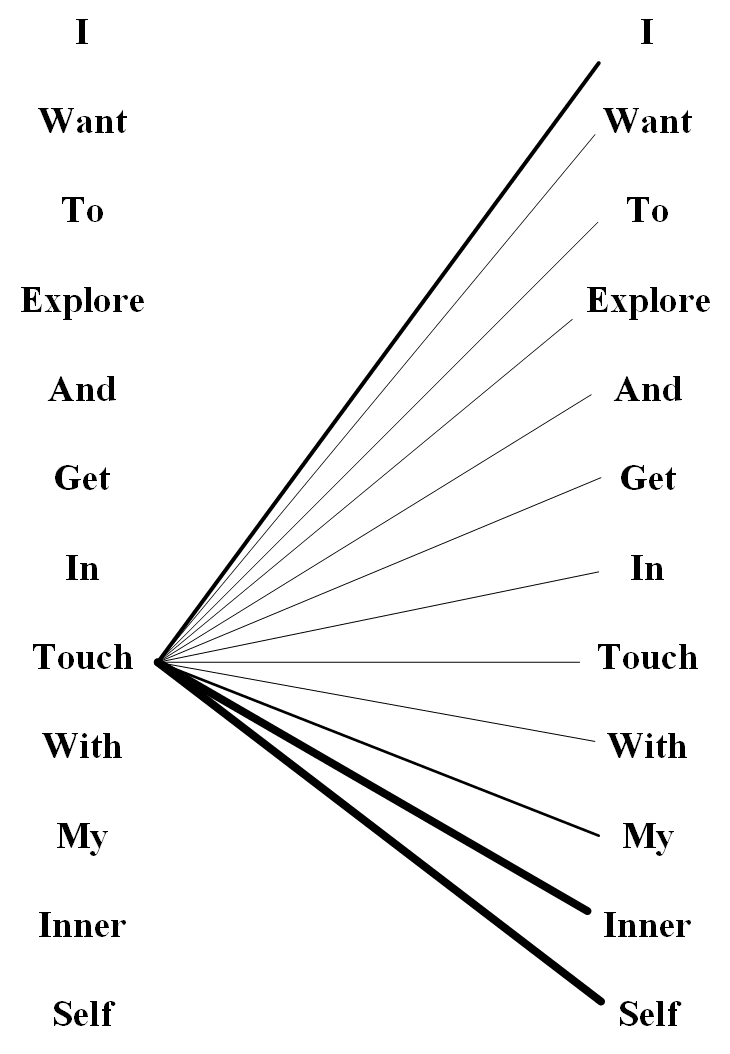
\includegraphics[width=0.4\textwidth]{pic/2-11.png}
	\caption{自注意力机制}
	\label{self-att}
\end{figure}
自注意力机制是一种关联单个序列的不同位置的注意力机制。通过计算每个位置与其他所有位置上的信息的注意力权重,从而获取得到对于当前位置最重要的一些信息,同时也能保留那些不重要的信息,更新当前位置的向量表示
。如图\ref{self-att}所示,单词‘touch’会计算所有其他单词的之间的注意力分数,分数大小由线段粗细为例,‘touch’可能更加关注于‘inner self’等单词,因此分配的权重也会更高,对于其他
单词分配的权重会低一些。Lin\citing{lin2017structured}采用注意力机制提出一个可解释性的文本嵌入模型,用于情感分析等任务上取得优异的结果。
\begin{figure}[htb]%\small tbp
	\setlength{\belowcaptionskip}{0pt}
	\centering
	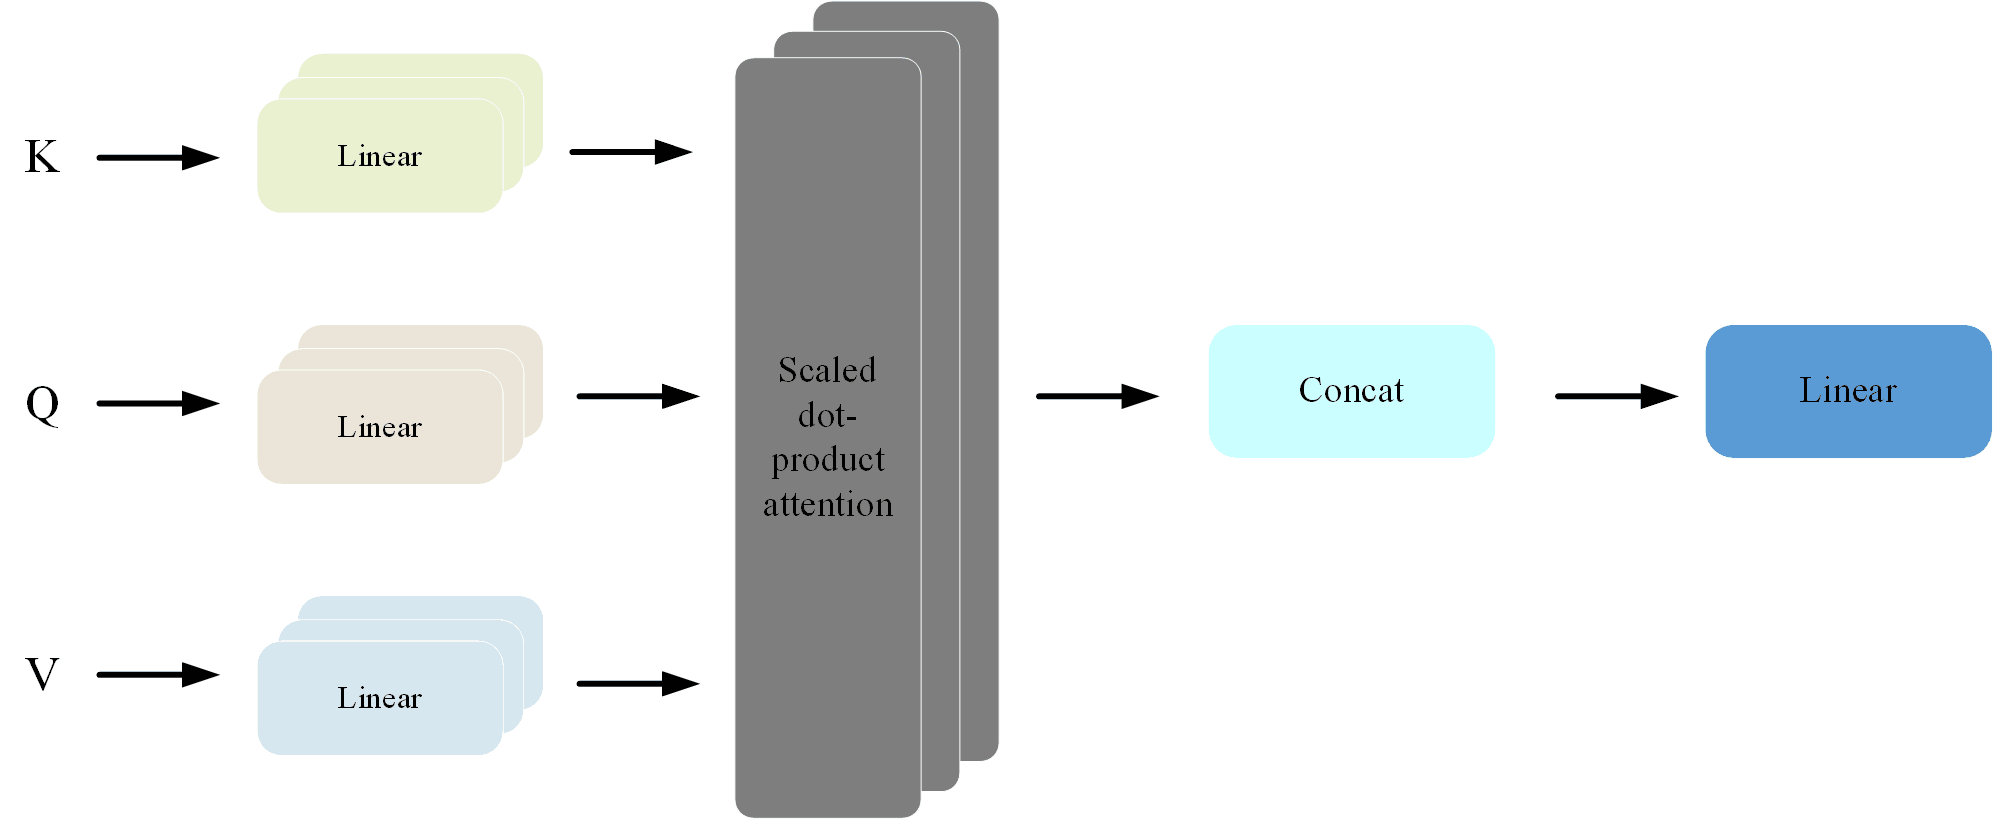
\includegraphics[width=0.8\textwidth]{pic/2-12.png}
	\caption{多头注意力机制}
	\label{muti-att}
\end{figure}

多头注意力机制首次由Vaswani\citing{vaswani2017attention}等人提出。首先将Query,Key,Value进行线性变换
,这里将计算多个线性变换,每个线性变换的参数均不一样。每一次的计算就是所谓的一个‘头’。然后采用放缩点积(scaled dot-Product attention)
方式计算,如公式\ref{scoreFormula3}所示。最后将结果拼接通过再通过一个线性变换层输出得到。如图\ref{muti-att}所示。
这样的好处就是可以允许模型在不同的表示子空间里学习到不同的相关信息。
\section{其他相关技术模型}
\subsection{TF-IDF}
TF-IDF是一种统计方法,用以评估一个字词对于一个文件集或一个语料库中的其中一份文件的重要程度。字词的重要性随着它在文件中出现的次数成正比增加,但同时会随着它在语料库中出现的频率成反比下降。
K. Sparck Jones\citing{jones1972statistical}提出了IDF的方法,这个方法可通过与词频连用以减少语料库中隐性常用词的影响。计算方法如公式\ref{idf}:
\begin{equation}\label{idf}
	idf=lg\frac{\left|D\right|}{\left|\{j:t_{i\ }\in d_j\}\right|}
\end{equation}

其中$D$表示语料库中的文件总数,分母包含单词$t_i$的文件数目。TF即是单词词频,表示如公式\ref{tf}所示:
\begin{equation}\label{tf}
	tf=\frac{n_i}{\sum n_k}
\end{equation}

其中$n_i$代表单词$i$出现的次数,分母为所有单词出现的总次数。TF-IDF联合使用,可以表示为:如果某个词或短语在一篇文章中出现的频率TF高,并且在其他文章中很少出现,则认为此词或者短语具有很好的类别区分能力。因此可以根据这个方法来做分类。

\subsection{CNN文本分类}
CNN(Convolutional Neural Networks)模型是一类包含卷积计算且具有深度结构的前馈神经网络(Feedforward Neural Networks),是深度学习(deep learning)的代表算法之一。卷积神经网络(CNN)具有表征学习能力,最主要的特征就是具有平移不变性。CNN最早可以追溯到日本科学家福岛邦彦\citing{fukushima1982neocognitron}提出的一个包含卷积层、池化层的神经网络结构。虽然中间消沉了一段时间,仅仅有一些少量性的研究工作,但Hinton等人提出的Alexnet\citing{krizhevsky2017imagenet},颠覆了图像识别领域,从而再次吸引了大量人员对于CNN的研究。
CNN主要应用于视频、图像等领域,由Kim等人\citing{kim2014convolutional}提出了Text-CNN模型,将CNN网络带入了文本处理领域。
\begin{figure}[htb]%\small tbp
	\setlength{\belowcaptionskip}{0pt}
	\centering
	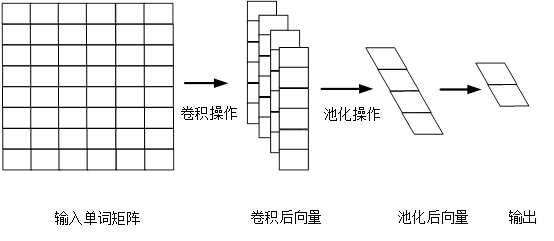
\includegraphics[width=0.8\textwidth]{pic/2-13.png}
	\caption{CNN模型}
	\label{cnn}
\end{figure}

如图\ref{cnn}所示,一段文本可以用一个$N\ast D$的矩阵表示,其中$N$代表文本中单词的数目,$D$代表单词向量的维度。经过一个$k\ast D$大小的卷积核操作,其中$k$表示为每次卷积操作的单词数,再经过一个池化层,得到一维向量表示。将多个卷积核操作获得的向量进行拼接,获得这段文本的向量表示。最后将这个向量表示输入一个分类器实现文本分类等任务。该CNN模型相比RNN模型,在一些比较的数据集来看,准确率相差不大,但是对于一些情感分类的文本来说有一定的优势。CNN最具优势的一点就是它能够并行计算,因而相比传统的RNN模型,计算速度有了较大提升,极大地缩短了训练时常,在一些比较注重实效的场景下,可以选择CNN模型。

\subsection{门控机制}
\begin{figure}[htb]%\small tbp
	\setlength{\belowcaptionskip}{0pt}
	\centering
	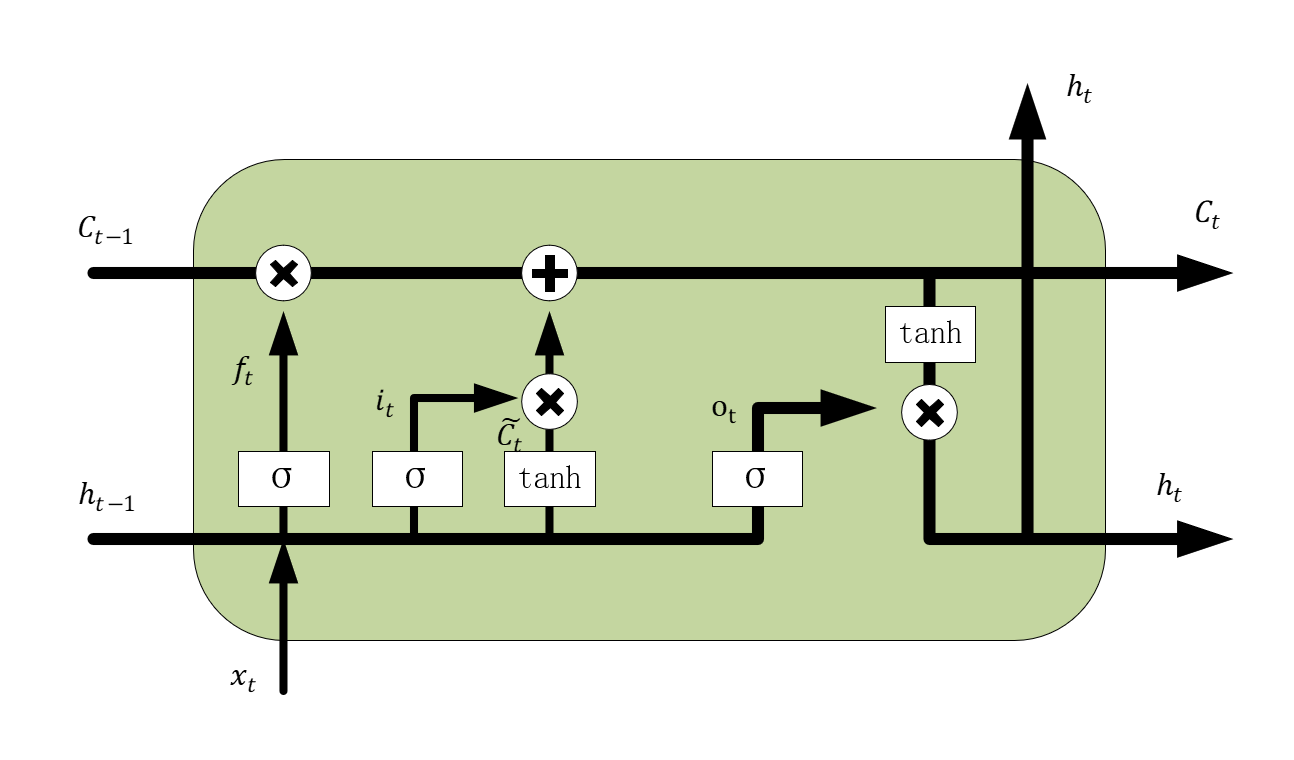
\includegraphics[width=0.8\textwidth]{pic/2-14.png}
	\caption{LSTM模型}
	\label{lstm}
\end{figure}
LSTM、GRU网络中采用了门控机制,实现了对短期记忆与长期记忆的结合,提升了模型性能,并且一定程度上解决了RNN模型的梯度消失问题。
如图\ref{lstm}所示,LSTM模型采用了门结构,门就是一个选择信息通过或抛弃的机制。计算过程如下:
\begin{equation}\label{LSTMFormula1}
	f_t=\sigma(W_f\bullet\left[h_{t-1},x_t\right]+b_f)
\end{equation}
\begin{equation}\label{LSTMFormula2}
	i_t=\sigma\left(W_i\bullet\left[h_{t-1},x_t\right]+b_i\right)
\end{equation}
\begin{equation}\label{LSTMFormula3}
	\widetilde{C_t}=tanh\left(W_c\bullet\left[h_{t-1},x_t\right]+b_c\right)
\end{equation}
\begin{equation}\label{LSTMFormula4}
	C_t=f_t\ast C_{t-1}+i_t\ast \widetilde{C_t}
\end{equation}
\begin{equation}\label{LSTMFormula5}
	o_t=\sigma\left(W_o\bullet\left[h_{t-1},x_t\right]+b_o\right)
\end{equation}
\begin{equation}\label{LSTMFormula6}
	h_t=o_t\ast tanh\left(C_t\right)
\end{equation}

LSTM中包含三个门结构,遗忘门、输入门以及输出门。遗忘门的计算首先通过之前的信息$h_{t-1}$以及当前输入信息$x_t$计算得到$f_t$,一个在0-1之前的数,用以选择哪些信息需要丢弃。随后再利用输入门计算$i_t$用以决定更新信息的量以及一个待选择的信息$\widetilde{C_t}$,最后计算出新的信息$C_t$。输出门利用$h_{t-1}$和$x_t$计算需要的特征,结合$C_t$信息,输出最终的向量表示$h_t$。该向量表示就可以代表整个文本的抽象特征,可以用来作文本分类任务。
\subsection{BERT模型}
BERT\citing{devlin2018bert}模型是基于transformer模型\citing{vaswani2017attention}提出的
\begin{figure}[htb]%\small tbp
	\setlength{\belowcaptionskip}{0pt}
	\centering
	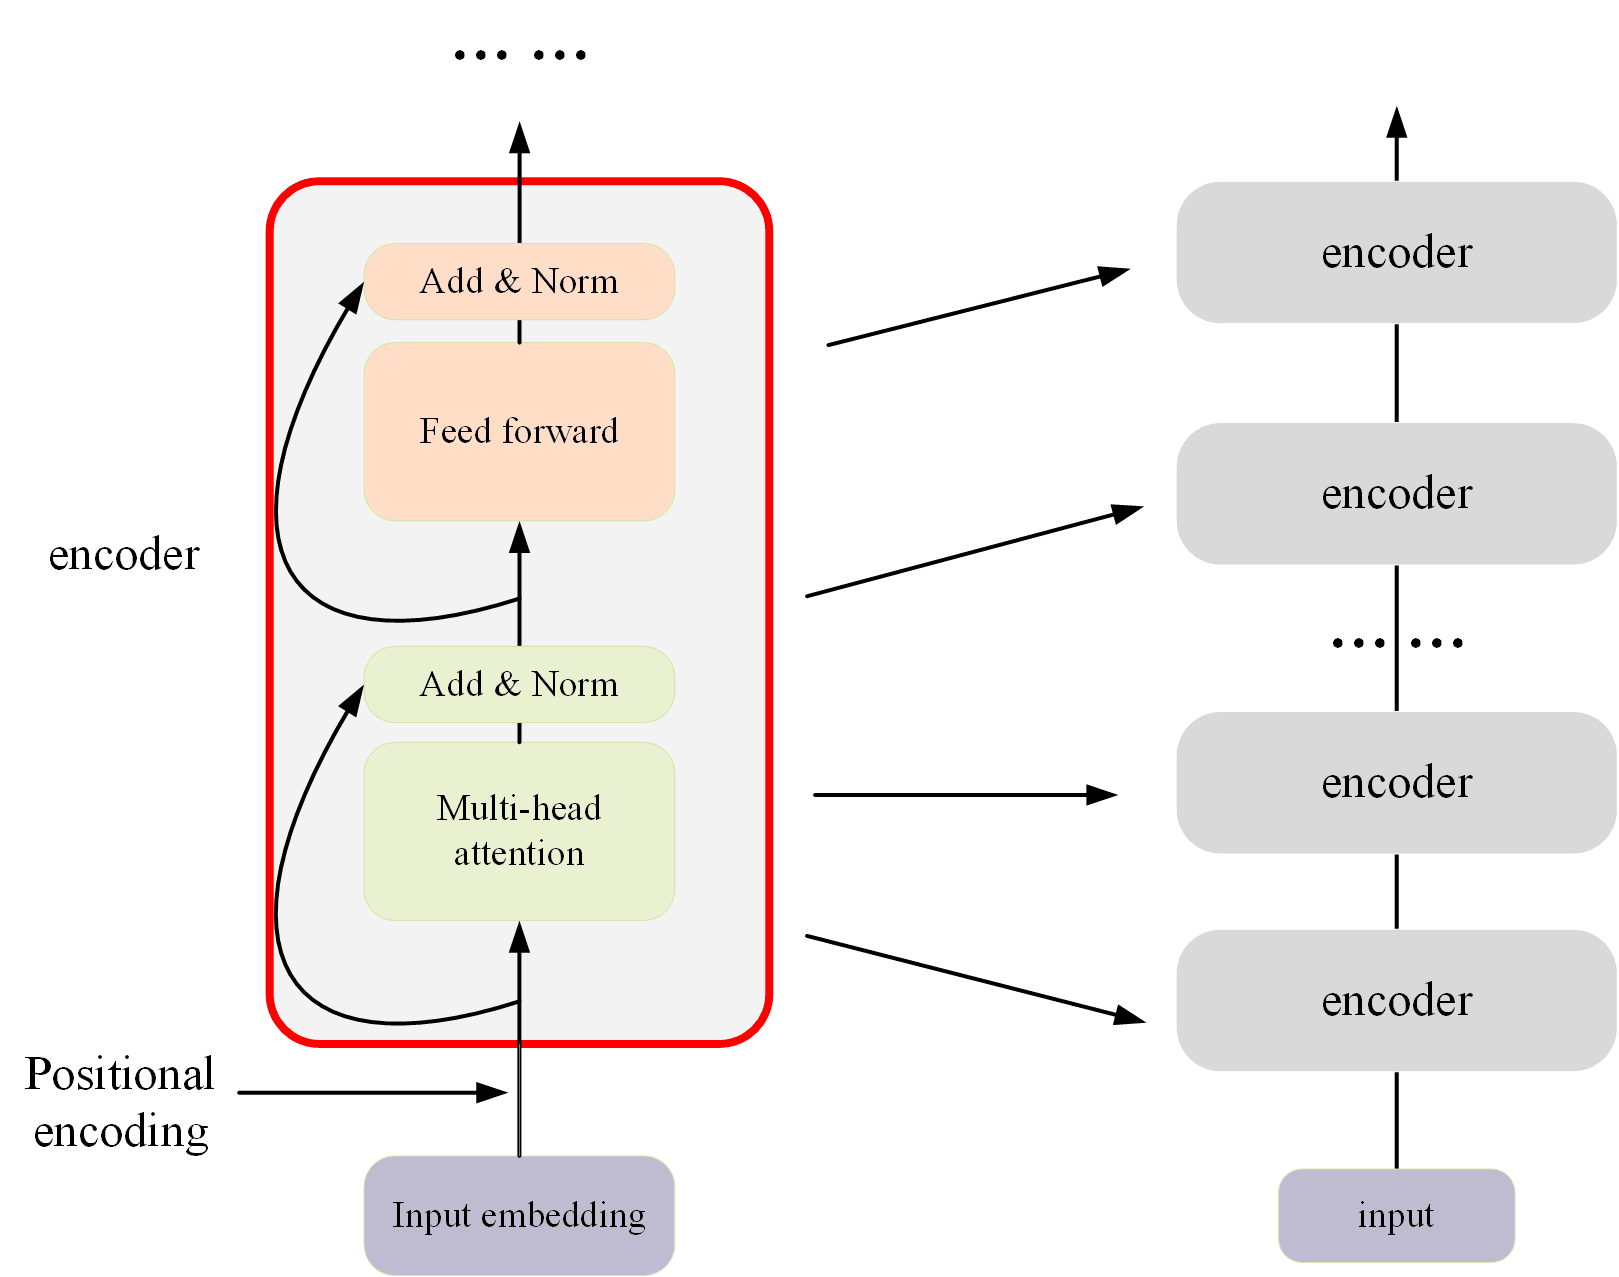
\includegraphics[width=0.8\textwidth]{pic/2-15.png}
	\caption{BERT模型基础架构}
	\label{bert}
\end{figure}
自然语言处理领域的预训练模型。如图\ref{bert}所示,bert主要结构采用了transformer的encoder部分,如图左所示。在每一个encoder结构中,
文本单词向量首先经过一个多头注意力机制以及一个残差连接的标准化层(add \& norm),之后在经过
线性转化和又一个标准化层,将结果输入到下一层网络。如图右所示,bert中由多个这样的encoder结构组成。
BERT预训练过程主要是随机遮盖或替换一句话里面任意字或词,然后让模型通过上下文的理解预测那一个被遮盖或替换的部分。

